\documentclass[twoside]{article}

% Packages required by doxygen
\usepackage{fixltx2e}
\usepackage{calc}
\usepackage{doxygen}
\usepackage[export]{adjustbox} % also loads graphicx
\usepackage{graphicx}
\usepackage[utf8]{inputenc}
\usepackage{makeidx}
\usepackage{multicol}
\usepackage{multirow}
\PassOptionsToPackage{warn}{textcomp}
\usepackage{textcomp}
\usepackage[nointegrals]{wasysym}
\usepackage[table]{xcolor}

% Font selection
\usepackage[T1]{fontenc}
\usepackage[scaled=.90]{helvet}
\usepackage{courier}
\usepackage{amssymb}
\usepackage{sectsty}
\renewcommand{\familydefault}{\sfdefault}
\allsectionsfont{%
  \fontseries{bc}\selectfont%
  \color{darkgray}%
}
\renewcommand{\DoxyLabelFont}{%
  \fontseries{bc}\selectfont%
  \color{darkgray}%
}
\newcommand{\+}{\discretionary{\mbox{\scriptsize$\hookleftarrow$}}{}{}}

% Page & text layout
\usepackage{geometry}
\geometry{%
  a4paper,%
  top=2.5cm,%
  bottom=2.5cm,%
  left=2.5cm,%
  right=2.5cm%
}
\tolerance=750
\hfuzz=15pt
\hbadness=750
\setlength{\emergencystretch}{15pt}
\setlength{\parindent}{0cm}
\setlength{\parskip}{3ex plus 2ex minus 2ex}
\makeatletter
\renewcommand{\paragraph}{%
  \@startsection{paragraph}{4}{0ex}{-1.0ex}{1.0ex}{%
    \normalfont\normalsize\bfseries\SS@parafont%
  }%
}
\renewcommand{\subparagraph}{%
  \@startsection{subparagraph}{5}{0ex}{-1.0ex}{1.0ex}{%
    \normalfont\normalsize\bfseries\SS@subparafont%
  }%
}
\makeatother

% Headers & footers
\usepackage{fancyhdr}
\pagestyle{fancyplain}
\fancyhead[LE]{\fancyplain{}{\bfseries\thepage}}
\fancyhead[CE]{\fancyplain{}{}}
\fancyhead[RE]{\fancyplain{}{\bfseries\leftmark}}
\fancyhead[LO]{\fancyplain{}{\bfseries\rightmark}}
\fancyhead[CO]{\fancyplain{}{}}
\fancyhead[RO]{\fancyplain{}{\bfseries\thepage}}
\fancyfoot[LE]{\fancyplain{}{}}
\fancyfoot[CE]{\fancyplain{}{}}
\fancyfoot[RE]{\fancyplain{}{\bfseries\scriptsize Generated by Doxygen }}
\fancyfoot[LO]{\fancyplain{}{\bfseries\scriptsize Generated by Doxygen }}
\fancyfoot[CO]{\fancyplain{}{}}
\fancyfoot[RO]{\fancyplain{}{}}
\renewcommand{\footrulewidth}{0.4pt}
\renewcommand{\sectionmark}[1]{%
  \markright{\thesection\ #1}%
}

% Indices & bibliography
\usepackage{natbib}
\usepackage[titles]{tocloft}
\setcounter{tocdepth}{3}
\setcounter{secnumdepth}{5}
\makeindex

% Hyperlinks (required, but should be loaded last)
\usepackage{ifpdf}
\ifpdf
  \usepackage[pdftex,pagebackref=true]{hyperref}
\else
  \usepackage[ps2pdf,pagebackref=true]{hyperref}
\fi
\hypersetup{%
  colorlinks=true,%
  linkcolor=blue,%
  citecolor=blue,%
  unicode%
}

% Custom commands
\newcommand{\clearemptydoublepage}{%
  \newpage{\pagestyle{empty}\cleardoublepage}%
}

\usepackage{caption}
\captionsetup{labelsep=space,justification=centering,font={bf},singlelinecheck=off,skip=4pt,position=top}

%===== C O N T E N T S =====

\begin{document}

% Titlepage & ToC
\hypersetup{pageanchor=false,
             bookmarksnumbered=true,
             pdfencoding=unicode
            }
\pagenumbering{alph}
\begin{titlepage}
\vspace*{7cm}
\begin{center}%
{\Large S\+T\+M32 Project }\\
\vspace*{1cm}
{\large Generated by Doxygen 1.8.13}\\
\end{center}
\end{titlepage}
\pagenumbering{roman}
\tableofcontents
\pagenumbering{arabic}
\hypersetup{pageanchor=true}

%--- Begin generated contents ---
\section{Hierarchical Index}
\subsection{Class Hierarchy}
This inheritance list is sorted roughly, but not completely, alphabetically\+:\begin{DoxyCompactList}
\item Q\+Chart\begin{DoxyCompactList}
\item \contentsline{section}{Chart}{\pageref{classChart}}{}
\end{DoxyCompactList}
\item Q\+Main\+Window\begin{DoxyCompactList}
\item \contentsline{section}{Main\+Window}{\pageref{classMainWindow}}{}
\end{DoxyCompactList}
\item Q\+Serial\+Port\begin{DoxyCompactList}
\item \contentsline{section}{Serial\+Port}{\pageref{classSerialPort}}{}
\end{DoxyCompactList}
\end{DoxyCompactList}

\section{Class Index}
\subsection{Class List}
Here are the classes, structs, unions and interfaces with brief descriptions\+:\begin{DoxyCompactList}
\item\contentsline{section}{\hyperlink{classChart}{Chart} }{\pageref{classChart}}{}
\item\contentsline{section}{\hyperlink{classMainWindow}{Main\+Window} }{\pageref{classMainWindow}}{}
\item\contentsline{section}{\hyperlink{classSerialPort}{Serial\+Port} }{\pageref{classSerialPort}}{}
\end{DoxyCompactList}

\section{File Index}
\section{File List}
Here is a list of all files with brief descriptions\+:\begin{DoxyCompactList}
\item\contentsline{section}{Inc/\hyperlink{main_8h}{main.\+h} \\*\+: Header for \hyperlink{main_8c}{main.\+c} file. This file contains the common defines of the application }{\pageref{main_8h}}{}
\item\contentsline{section}{Inc/\hyperlink{stm32f3xx__hal__conf_8h}{stm32f3xx\+\_\+hal\+\_\+conf.\+h} \\*H\+AL configuration file }{\pageref{stm32f3xx__hal__conf_8h}}{}
\item\contentsline{section}{Inc/\hyperlink{stm32f3xx__it_8h}{stm32f3xx\+\_\+it.\+h} \\*This file contains the headers of the interrupt handlers }{\pageref{stm32f3xx__it_8h}}{}
\item\contentsline{section}{Src/\hyperlink{main_8c}{main.\+c} \\*\+: Main program body }{\pageref{main_8c}}{}
\item\contentsline{section}{Src/\hyperlink{stm32f3xx__hal__msp_8c}{stm32f3xx\+\_\+hal\+\_\+msp.\+c} }{\pageref{stm32f3xx__hal__msp_8c}}{}
\item\contentsline{section}{Src/\hyperlink{stm32f3xx__it_8c}{stm32f3xx\+\_\+it.\+c} \\*Interrupt Service Routines }{\pageref{stm32f3xx__it_8c}}{}
\item\contentsline{section}{Src/\hyperlink{system__stm32f3xx_8c}{system\+\_\+stm32f3xx.\+c} \\*C\+M\+S\+IS Cortex-\/\+M4 Device Peripheral Access Layer System Source File }{\pageref{system__stm32f3xx_8c}}{}
\end{DoxyCompactList}

\section{Class Documentation}
\hypertarget{classChart}{}\subsection{Chart Class Reference}
\label{classChart}\index{Chart@{Chart}}


{\ttfamily \#include $<$Chart.\+h$>$}



Inheritance diagram for Chart\+:\nopagebreak
\begin{figure}[H]
\begin{center}
\leavevmode
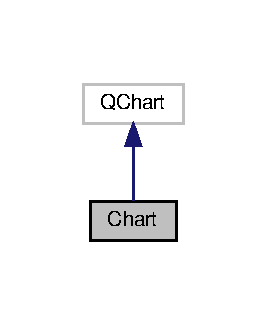
\includegraphics[width=128pt]{classChart__inherit__graph}
\end{center}
\end{figure}


Collaboration diagram for Chart\+:\nopagebreak
\begin{figure}[H]
\begin{center}
\leavevmode
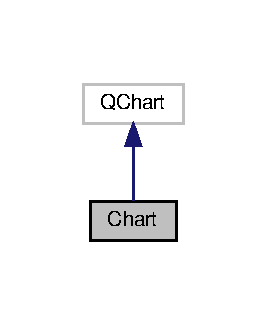
\includegraphics[width=128pt]{classChart__coll__graph}
\end{center}
\end{figure}
\subsubsection*{Public Slots}
\begin{DoxyCompactItemize}
\item 
void \hyperlink{classChart_abefbafd5e6582e649d40444d16331b94}{add\+Data} (Q\+String str)
\begin{DoxyCompactList}\small\item\em Receives values and add them. \end{DoxyCompactList}\end{DoxyCompactItemize}
\subsubsection*{Public Member Functions}
\begin{DoxyCompactItemize}
\item 
\hyperlink{classChart_a61896fddeb02818af2892cb6d9cdadb4}{Chart} ()
\begin{DoxyCompactList}\small\item\em Sets up basic parameters. \end{DoxyCompactList}\item 
void \hyperlink{classChart_a445baba8efcb1c0bea7f7f16e2d5b1e9}{set\+Range} (int range)
\begin{DoxyCompactList}\small\item\em Sets range. \end{DoxyCompactList}\item 
void \hyperlink{classChart_af996c93e298c33c8eeaead89d9933c15}{set\+Measurement\+Rate} (int rate)
\begin{DoxyCompactList}\small\item\em Sets measurement rate. \end{DoxyCompactList}\item 
void \hyperlink{classChart_a1bf5a87044118c780a83b1ff03428374}{clear} ()
\begin{DoxyCompactList}\small\item\em Clears series and set (x,y) to zero. \end{DoxyCompactList}\item 
float \hyperlink{classChart_a0636026f9baa6bbdc51a83fdad4db109}{get\+Measurement\+Rate} ()
\begin{DoxyCompactList}\small\item\em Currently doesn\textquotesingle{}t matter. \end{DoxyCompactList}\end{DoxyCompactItemize}
\subsubsection*{Private Attributes}
\begin{DoxyCompactItemize}
\item 
std\+::unique\+\_\+ptr$<$ Q\+Elapsed\+Timer $>$ \hyperlink{classChart_a586658c9f0ef3a3bd5d614a178436865}{\+\_\+timer}
\item 
float \hyperlink{classChart_a714191d2fc69d06d66872bba187d144b}{\+\_\+x\+Range}
\item 
float \hyperlink{classChart_a5434effc2361d5f6890982e83e8bc871}{\+\_\+x\+Current}
\item 
float \hyperlink{classChart_a7034a9d00d36ee96eb8af2d7c2af832d}{\+\_\+x\+Measurement\+Rate}
\item 
float \hyperlink{classChart_aeac5778c508d702f8deb07cbb7b2c867}{\+\_\+y\+Max}
\item 
std\+::unique\+\_\+ptr$<$ Q\+Line\+Series $>$ \hyperlink{classChart_a2b6b5680d382cb18164593293825fc08}{\+\_\+series}
\end{DoxyCompactItemize}


\subsubsection{Constructor \& Destructor Documentation}
\mbox{\Hypertarget{classChart_a61896fddeb02818af2892cb6d9cdadb4}\label{classChart_a61896fddeb02818af2892cb6d9cdadb4}} 
\index{Chart@{Chart}!Chart@{Chart}}
\index{Chart@{Chart}!Chart@{Chart}}
\paragraph{\texorpdfstring{Chart()}{Chart()}}
{\footnotesize\ttfamily Chart\+::\+Chart (\begin{DoxyParamCaption}{ }\end{DoxyParamCaption})}



Sets up basic parameters. 



\subsubsection{Member Function Documentation}
\mbox{\Hypertarget{classChart_abefbafd5e6582e649d40444d16331b94}\label{classChart_abefbafd5e6582e649d40444d16331b94}} 
\index{Chart@{Chart}!add\+Data@{add\+Data}}
\index{add\+Data@{add\+Data}!Chart@{Chart}}
\paragraph{\texorpdfstring{add\+Data}{addData}}
{\footnotesize\ttfamily void Chart\+::add\+Data (\begin{DoxyParamCaption}\item[{Q\+String}]{str }\end{DoxyParamCaption})\hspace{0.3cm}{\ttfamily [slot]}}



Receives values and add them. 


\begin{DoxyParams}{Parameters}
{\em str} & it\textquotesingle{}s Q\+String with received value \\
\hline
\end{DoxyParams}
\mbox{\Hypertarget{classChart_a1bf5a87044118c780a83b1ff03428374}\label{classChart_a1bf5a87044118c780a83b1ff03428374}} 
\index{Chart@{Chart}!clear@{clear}}
\index{clear@{clear}!Chart@{Chart}}
\paragraph{\texorpdfstring{clear()}{clear()}}
{\footnotesize\ttfamily void Chart\+::clear (\begin{DoxyParamCaption}{ }\end{DoxyParamCaption})}



Clears series and set (x,y) to zero. 

\mbox{\Hypertarget{classChart_a0636026f9baa6bbdc51a83fdad4db109}\label{classChart_a0636026f9baa6bbdc51a83fdad4db109}} 
\index{Chart@{Chart}!get\+Measurement\+Rate@{get\+Measurement\+Rate}}
\index{get\+Measurement\+Rate@{get\+Measurement\+Rate}!Chart@{Chart}}
\paragraph{\texorpdfstring{get\+Measurement\+Rate()}{getMeasurementRate()}}
{\footnotesize\ttfamily float Chart\+::get\+Measurement\+Rate (\begin{DoxyParamCaption}{ }\end{DoxyParamCaption})}



Currently doesn\textquotesingle{}t matter. 

\begin{DoxyReturn}{Returns}
returns set value of measurement rate 
\end{DoxyReturn}
\mbox{\Hypertarget{classChart_af996c93e298c33c8eeaead89d9933c15}\label{classChart_af996c93e298c33c8eeaead89d9933c15}} 
\index{Chart@{Chart}!set\+Measurement\+Rate@{set\+Measurement\+Rate}}
\index{set\+Measurement\+Rate@{set\+Measurement\+Rate}!Chart@{Chart}}
\paragraph{\texorpdfstring{set\+Measurement\+Rate()}{setMeasurementRate()}}
{\footnotesize\ttfamily void Chart\+::set\+Measurement\+Rate (\begin{DoxyParamCaption}\item[{int}]{rate }\end{DoxyParamCaption})}



Sets measurement rate. 


\begin{DoxyParams}{Parameters}
{\em rate} & \\
\hline
\end{DoxyParams}
\mbox{\Hypertarget{classChart_a445baba8efcb1c0bea7f7f16e2d5b1e9}\label{classChart_a445baba8efcb1c0bea7f7f16e2d5b1e9}} 
\index{Chart@{Chart}!set\+Range@{set\+Range}}
\index{set\+Range@{set\+Range}!Chart@{Chart}}
\paragraph{\texorpdfstring{set\+Range()}{setRange()}}
{\footnotesize\ttfamily void Chart\+::set\+Range (\begin{DoxyParamCaption}\item[{int}]{range }\end{DoxyParamCaption})}



Sets range. 


\begin{DoxyParams}{Parameters}
{\em range} & \\
\hline
\end{DoxyParams}


\subsubsection{Member Data Documentation}
\mbox{\Hypertarget{classChart_a2b6b5680d382cb18164593293825fc08}\label{classChart_a2b6b5680d382cb18164593293825fc08}} 
\index{Chart@{Chart}!\+\_\+series@{\+\_\+series}}
\index{\+\_\+series@{\+\_\+series}!Chart@{Chart}}
\paragraph{\texorpdfstring{\+\_\+series}{\_series}}
{\footnotesize\ttfamily std\+::unique\+\_\+ptr$<$Q\+Line\+Series$>$ Chart\+::\+\_\+series\hspace{0.3cm}{\ttfamily [private]}}

\mbox{\Hypertarget{classChart_a586658c9f0ef3a3bd5d614a178436865}\label{classChart_a586658c9f0ef3a3bd5d614a178436865}} 
\index{Chart@{Chart}!\+\_\+timer@{\+\_\+timer}}
\index{\+\_\+timer@{\+\_\+timer}!Chart@{Chart}}
\paragraph{\texorpdfstring{\+\_\+timer}{\_timer}}
{\footnotesize\ttfamily std\+::unique\+\_\+ptr$<$Q\+Elapsed\+Timer$>$ Chart\+::\+\_\+timer\hspace{0.3cm}{\ttfamily [private]}}

\mbox{\Hypertarget{classChart_a5434effc2361d5f6890982e83e8bc871}\label{classChart_a5434effc2361d5f6890982e83e8bc871}} 
\index{Chart@{Chart}!\+\_\+x\+Current@{\+\_\+x\+Current}}
\index{\+\_\+x\+Current@{\+\_\+x\+Current}!Chart@{Chart}}
\paragraph{\texorpdfstring{\+\_\+x\+Current}{\_xCurrent}}
{\footnotesize\ttfamily float Chart\+::\+\_\+x\+Current\hspace{0.3cm}{\ttfamily [private]}}

\mbox{\Hypertarget{classChart_a7034a9d00d36ee96eb8af2d7c2af832d}\label{classChart_a7034a9d00d36ee96eb8af2d7c2af832d}} 
\index{Chart@{Chart}!\+\_\+x\+Measurement\+Rate@{\+\_\+x\+Measurement\+Rate}}
\index{\+\_\+x\+Measurement\+Rate@{\+\_\+x\+Measurement\+Rate}!Chart@{Chart}}
\paragraph{\texorpdfstring{\+\_\+x\+Measurement\+Rate}{\_xMeasurementRate}}
{\footnotesize\ttfamily float Chart\+::\+\_\+x\+Measurement\+Rate\hspace{0.3cm}{\ttfamily [private]}}

\mbox{\Hypertarget{classChart_a714191d2fc69d06d66872bba187d144b}\label{classChart_a714191d2fc69d06d66872bba187d144b}} 
\index{Chart@{Chart}!\+\_\+x\+Range@{\+\_\+x\+Range}}
\index{\+\_\+x\+Range@{\+\_\+x\+Range}!Chart@{Chart}}
\paragraph{\texorpdfstring{\+\_\+x\+Range}{\_xRange}}
{\footnotesize\ttfamily float Chart\+::\+\_\+x\+Range\hspace{0.3cm}{\ttfamily [private]}}

\mbox{\Hypertarget{classChart_aeac5778c508d702f8deb07cbb7b2c867}\label{classChart_aeac5778c508d702f8deb07cbb7b2c867}} 
\index{Chart@{Chart}!\+\_\+y\+Max@{\+\_\+y\+Max}}
\index{\+\_\+y\+Max@{\+\_\+y\+Max}!Chart@{Chart}}
\paragraph{\texorpdfstring{\+\_\+y\+Max}{\_yMax}}
{\footnotesize\ttfamily float Chart\+::\+\_\+y\+Max\hspace{0.3cm}{\ttfamily [private]}}



The documentation for this class was generated from the following files\+:\begin{DoxyCompactItemize}
\item 
\hyperlink{Chart_8h}{Chart.\+h}\item 
\hyperlink{Chart_8cpp}{Chart.\+cpp}\end{DoxyCompactItemize}

\hypertarget{classMainWindow}{}\subsection{Main\+Window Class Reference}
\label{classMainWindow}\index{Main\+Window@{Main\+Window}}


{\ttfamily \#include $<$mainwindow.\+h$>$}



Inheritance diagram for Main\+Window\+:\nopagebreak
\begin{figure}[H]
\begin{center}
\leavevmode
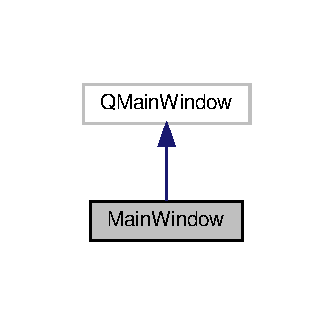
\includegraphics[width=160pt]{classMainWindow__inherit__graph}
\end{center}
\end{figure}


Collaboration diagram for Main\+Window\+:\nopagebreak
\begin{figure}[H]
\begin{center}
\leavevmode
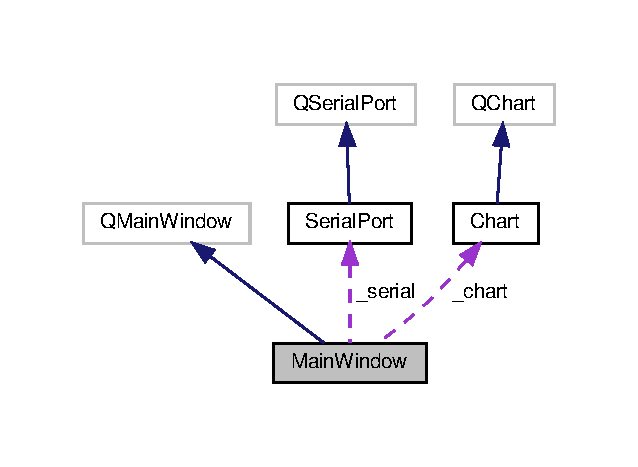
\includegraphics[width=306pt]{classMainWindow__coll__graph}
\end{center}
\end{figure}
\subsubsection*{Public Member Functions}
\begin{DoxyCompactItemize}
\item 
\hyperlink{classMainWindow_a8b244be8b7b7db1b08de2a2acb9409db}{Main\+Window} (Q\+Widget $\ast$parent=0)
\begin{DoxyCompactList}\small\item\em Sets up basic parameters. \end{DoxyCompactList}\item 
\hyperlink{classMainWindow_ae98d00a93bc118200eeef9f9bba1dba7}{$\sim$\+Main\+Window} ()
\begin{DoxyCompactList}\small\item\em Destroys all pointers. \end{DoxyCompactList}\end{DoxyCompactItemize}
\subsubsection*{Private Slots}
\begin{DoxyCompactItemize}
\item 
void \hyperlink{classMainWindow_a22d5b63d63ca5fc1fb9a7ef40efc38c8}{open\+Serial\+Port} ()
\begin{DoxyCompactList}\small\item\em Tries to connect to serial port. \end{DoxyCompactList}\item 
void \hyperlink{classMainWindow_ac5eae1a5faf30bb616185aa3be724484}{close\+Serial\+Port} ()
\begin{DoxyCompactList}\small\item\em Closes connection to serial port. \end{DoxyCompactList}\item 
void \hyperlink{classMainWindow_a76237574ac5c68506bcb9b9de468fda2}{write\+Data} (const Q\+Byte\+Array \&data)
\begin{DoxyCompactList}\small\item\em Sends data through serial port. \end{DoxyCompactList}\item 
void \hyperlink{classMainWindow_a5afc1f8c3bbce5e91e4cebf2dd4e6069}{search\+For\+Ports} ()
\begin{DoxyCompactList}\small\item\em Search for ports. \end{DoxyCompactList}\item 
void \hyperlink{classMainWindow_ad7ece63fdbb09608a22fc0631143b6ec}{line\+Edit\+Enter\+Text} ()
\begin{DoxyCompactList}\small\item\em Sends data. \end{DoxyCompactList}\item 
void \hyperlink{classMainWindow_ad3fa656a0c81fa2ec687b02bd0f9658b}{measurement\+Changed} (int index)
\begin{DoxyCompactList}\small\item\em Changes measurement goal. \end{DoxyCompactList}\item 
void \hyperlink{classMainWindow_a89b2e9afba74a68fd3b4a28d4475cec7}{plain\+Text\+Changed} ()
\begin{DoxyCompactList}\small\item\em Scrolls to bottom when required. \end{DoxyCompactList}\item 
void \hyperlink{classMainWindow_a19690cb09dbe0abd4252c6b8236d6810}{handle\+Error} (Q\+Serial\+Port\+::\+Serial\+Port\+Error error)
\begin{DoxyCompactList}\small\item\em Display all errors. \end{DoxyCompactList}\item 
void \hyperlink{classMainWindow_a922a5c49b11ae3ec01663b409cfc35c1}{button\+Clicked} ()
\begin{DoxyCompactList}\small\item\em Handles connection\textquotesingle{}s button. \end{DoxyCompactList}\end{DoxyCompactItemize}
\subsubsection*{Private Member Functions}
\begin{DoxyCompactItemize}
\item 
Q\+Grid\+Layout $\ast$ \hyperlink{classMainWindow_a19f1d3f1ccdc04be0f5f63f0c99264f4}{setup\+Main\+Layout} ()
\begin{DoxyCompactList}\small\item\em Sets up whole layout. \end{DoxyCompactList}\item 
void \hyperlink{classMainWindow_a74ab7a387068bddadc3e665ba64b73b8}{setup\+Serial} ()
\begin{DoxyCompactList}\small\item\em Sets up all required values for serial connection. \end{DoxyCompactList}\item 
void \hyperlink{classMainWindow_a5235529d74723de1e3686da400dd1d37}{init\+Actions\+Connections} ()
\begin{DoxyCompactList}\small\item\em Initializes all connections. \end{DoxyCompactList}\end{DoxyCompactItemize}
\subsubsection*{Private Attributes}
\begin{DoxyCompactItemize}
\item 
\hyperlink{classChart}{Chart} $\ast$ \hyperlink{classMainWindow_abceb3cc9b41fa17bf367f7cb475a0a03}{\+\_\+chart}
\item 
\hyperlink{classSerialPort}{Serial\+Port} $\ast$ \hyperlink{classMainWindow_a19f91aa8908f303c76ce28b091f97e73}{\+\_\+serial}
\item 
Q\+Push\+Button $\ast$ \hyperlink{classMainWindow_a8a24c0fa7a9ce08d7c62043cb90c1a84}{\+\_\+connect\+Btn}
\item 
Q\+Push\+Button $\ast$ \hyperlink{classMainWindow_a8de7f487a7dfb1d7e7d15e3a1366fa15}{\+\_\+refresh\+Btn}
\item 
Q\+Plain\+Text\+Edit $\ast$ \hyperlink{classMainWindow_aad53a19d55400715e21a8c4a94cd6754}{\+\_\+plain}
\item 
Q\+Chart\+View $\ast$ \hyperlink{classMainWindow_a5c1071e1a9b436f607e14dd85cc51c6f}{\+\_\+chart\+View}
\item 
Q\+Combo\+Box $\ast$ \hyperlink{classMainWindow_a4412056949abeb7a14a44491be5fc9ea}{\+\_\+port\+Box}
\item 
Q\+Combo\+Box $\ast$ \hyperlink{classMainWindow_aff8ced34c2938264052e888fa31c9704}{\+\_\+baud\+Rate\+Box}
\item 
Q\+Combo\+Box $\ast$ \hyperlink{classMainWindow_ae6041d00d855eaa9f8a03297c556465a}{\+\_\+parity\+Box}
\item 
Q\+Combo\+Box $\ast$ \hyperlink{classMainWindow_ad886195377aedece39671edd11ed5d39}{\+\_\+stop\+Bits\+Box}
\item 
Q\+Combo\+Box $\ast$ \hyperlink{classMainWindow_ac4ca89e6458dbce1f4dca70f17123892}{\+\_\+flow\+Control\+Box}
\item 
Q\+Combo\+Box $\ast$ \hyperlink{classMainWindow_a9ebbfaef63c626558fd9ecca791493a6}{\+\_\+measurement\+Box}
\item 
Q\+Spin\+Box $\ast$ \hyperlink{classMainWindow_ab5c9c33a5b95515303a7aabdf05e70b1}{\+\_\+spin\+Box}
\item 
Q\+Label $\ast$ \hyperlink{classMainWindow_a1b4b4e9cd06c11051d9d88c17334b57e}{\+\_\+label}
\item 
Q\+Line\+Edit $\ast$ \hyperlink{classMainWindow_ad8d180d000764830c6600213928fa38d}{\+\_\+line\+Edit}
\item 
Q\+Check\+Box $\ast$ \hyperlink{classMainWindow_aacb799cbf321719bbb1d682302798252}{\+\_\+auto\+Scroll\+Box}
\end{DoxyCompactItemize}


\subsubsection{Detailed Description}
\begin{DoxyAuthor}{Author}
Przemyslaw Papla 
\end{DoxyAuthor}


\subsubsection{Constructor \& Destructor Documentation}
\mbox{\Hypertarget{classMainWindow_a8b244be8b7b7db1b08de2a2acb9409db}\label{classMainWindow_a8b244be8b7b7db1b08de2a2acb9409db}} 
\index{Main\+Window@{Main\+Window}!Main\+Window@{Main\+Window}}
\index{Main\+Window@{Main\+Window}!Main\+Window@{Main\+Window}}
\paragraph{\texorpdfstring{Main\+Window()}{MainWindow()}}
{\footnotesize\ttfamily Main\+Window\+::\+Main\+Window (\begin{DoxyParamCaption}\item[{Q\+Widget $\ast$}]{parent = {\ttfamily 0} }\end{DoxyParamCaption})\hspace{0.3cm}{\ttfamily [explicit]}}



Sets up basic parameters. 


\begin{DoxyParams}{Parameters}
{\em parent} & \\
\hline
\end{DoxyParams}
\mbox{\Hypertarget{classMainWindow_ae98d00a93bc118200eeef9f9bba1dba7}\label{classMainWindow_ae98d00a93bc118200eeef9f9bba1dba7}} 
\index{Main\+Window@{Main\+Window}!````~Main\+Window@{$\sim$\+Main\+Window}}
\index{````~Main\+Window@{$\sim$\+Main\+Window}!Main\+Window@{Main\+Window}}
\paragraph{\texorpdfstring{$\sim$\+Main\+Window()}{~MainWindow()}}
{\footnotesize\ttfamily Main\+Window\+::$\sim$\+Main\+Window (\begin{DoxyParamCaption}{ }\end{DoxyParamCaption})}



Destroys all pointers. 



\subsubsection{Member Function Documentation}
\mbox{\Hypertarget{classMainWindow_a922a5c49b11ae3ec01663b409cfc35c1}\label{classMainWindow_a922a5c49b11ae3ec01663b409cfc35c1}} 
\index{Main\+Window@{Main\+Window}!button\+Clicked@{button\+Clicked}}
\index{button\+Clicked@{button\+Clicked}!Main\+Window@{Main\+Window}}
\paragraph{\texorpdfstring{button\+Clicked}{buttonClicked}}
{\footnotesize\ttfamily void Main\+Window\+::button\+Clicked (\begin{DoxyParamCaption}{ }\end{DoxyParamCaption})\hspace{0.3cm}{\ttfamily [private]}, {\ttfamily [slot]}}



Handles connection\textquotesingle{}s button. 

\mbox{\Hypertarget{classMainWindow_ac5eae1a5faf30bb616185aa3be724484}\label{classMainWindow_ac5eae1a5faf30bb616185aa3be724484}} 
\index{Main\+Window@{Main\+Window}!close\+Serial\+Port@{close\+Serial\+Port}}
\index{close\+Serial\+Port@{close\+Serial\+Port}!Main\+Window@{Main\+Window}}
\paragraph{\texorpdfstring{close\+Serial\+Port}{closeSerialPort}}
{\footnotesize\ttfamily void Main\+Window\+::close\+Serial\+Port (\begin{DoxyParamCaption}{ }\end{DoxyParamCaption})\hspace{0.3cm}{\ttfamily [private]}, {\ttfamily [slot]}}



Closes connection to serial port. 

\mbox{\Hypertarget{classMainWindow_a19690cb09dbe0abd4252c6b8236d6810}\label{classMainWindow_a19690cb09dbe0abd4252c6b8236d6810}} 
\index{Main\+Window@{Main\+Window}!handle\+Error@{handle\+Error}}
\index{handle\+Error@{handle\+Error}!Main\+Window@{Main\+Window}}
\paragraph{\texorpdfstring{handle\+Error}{handleError}}
{\footnotesize\ttfamily void Main\+Window\+::handle\+Error (\begin{DoxyParamCaption}\item[{Q\+Serial\+Port\+::\+Serial\+Port\+Error}]{error }\end{DoxyParamCaption})\hspace{0.3cm}{\ttfamily [private]}, {\ttfamily [slot]}}



Display all errors. 


\begin{DoxyParams}{Parameters}
{\em error} & \\
\hline
\end{DoxyParams}
\mbox{\Hypertarget{classMainWindow_a5235529d74723de1e3686da400dd1d37}\label{classMainWindow_a5235529d74723de1e3686da400dd1d37}} 
\index{Main\+Window@{Main\+Window}!init\+Actions\+Connections@{init\+Actions\+Connections}}
\index{init\+Actions\+Connections@{init\+Actions\+Connections}!Main\+Window@{Main\+Window}}
\paragraph{\texorpdfstring{init\+Actions\+Connections()}{initActionsConnections()}}
{\footnotesize\ttfamily void Main\+Window\+::init\+Actions\+Connections (\begin{DoxyParamCaption}{ }\end{DoxyParamCaption})\hspace{0.3cm}{\ttfamily [private]}}



Initializes all connections. 

\mbox{\Hypertarget{classMainWindow_ad7ece63fdbb09608a22fc0631143b6ec}\label{classMainWindow_ad7ece63fdbb09608a22fc0631143b6ec}} 
\index{Main\+Window@{Main\+Window}!line\+Edit\+Enter\+Text@{line\+Edit\+Enter\+Text}}
\index{line\+Edit\+Enter\+Text@{line\+Edit\+Enter\+Text}!Main\+Window@{Main\+Window}}
\paragraph{\texorpdfstring{line\+Edit\+Enter\+Text}{lineEditEnterText}}
{\footnotesize\ttfamily void Main\+Window\+::line\+Edit\+Enter\+Text (\begin{DoxyParamCaption}{ }\end{DoxyParamCaption})\hspace{0.3cm}{\ttfamily [private]}, {\ttfamily [slot]}}



Sends data. 

\mbox{\Hypertarget{classMainWindow_ad3fa656a0c81fa2ec687b02bd0f9658b}\label{classMainWindow_ad3fa656a0c81fa2ec687b02bd0f9658b}} 
\index{Main\+Window@{Main\+Window}!measurement\+Changed@{measurement\+Changed}}
\index{measurement\+Changed@{measurement\+Changed}!Main\+Window@{Main\+Window}}
\paragraph{\texorpdfstring{measurement\+Changed}{measurementChanged}}
{\footnotesize\ttfamily void Main\+Window\+::measurement\+Changed (\begin{DoxyParamCaption}\item[{int}]{index }\end{DoxyParamCaption})\hspace{0.3cm}{\ttfamily [private]}, {\ttfamily [slot]}}



Changes measurement goal. 


\begin{DoxyParams}{Parameters}
{\em index} & \\
\hline
\end{DoxyParams}
\mbox{\Hypertarget{classMainWindow_a22d5b63d63ca5fc1fb9a7ef40efc38c8}\label{classMainWindow_a22d5b63d63ca5fc1fb9a7ef40efc38c8}} 
\index{Main\+Window@{Main\+Window}!open\+Serial\+Port@{open\+Serial\+Port}}
\index{open\+Serial\+Port@{open\+Serial\+Port}!Main\+Window@{Main\+Window}}
\paragraph{\texorpdfstring{open\+Serial\+Port}{openSerialPort}}
{\footnotesize\ttfamily void Main\+Window\+::open\+Serial\+Port (\begin{DoxyParamCaption}{ }\end{DoxyParamCaption})\hspace{0.3cm}{\ttfamily [private]}, {\ttfamily [slot]}}



Tries to connect to serial port. 

\mbox{\Hypertarget{classMainWindow_a89b2e9afba74a68fd3b4a28d4475cec7}\label{classMainWindow_a89b2e9afba74a68fd3b4a28d4475cec7}} 
\index{Main\+Window@{Main\+Window}!plain\+Text\+Changed@{plain\+Text\+Changed}}
\index{plain\+Text\+Changed@{plain\+Text\+Changed}!Main\+Window@{Main\+Window}}
\paragraph{\texorpdfstring{plain\+Text\+Changed}{plainTextChanged}}
{\footnotesize\ttfamily void Main\+Window\+::plain\+Text\+Changed (\begin{DoxyParamCaption}{ }\end{DoxyParamCaption})\hspace{0.3cm}{\ttfamily [private]}, {\ttfamily [slot]}}



Scrolls to bottom when required. 

\mbox{\Hypertarget{classMainWindow_a5afc1f8c3bbce5e91e4cebf2dd4e6069}\label{classMainWindow_a5afc1f8c3bbce5e91e4cebf2dd4e6069}} 
\index{Main\+Window@{Main\+Window}!search\+For\+Ports@{search\+For\+Ports}}
\index{search\+For\+Ports@{search\+For\+Ports}!Main\+Window@{Main\+Window}}
\paragraph{\texorpdfstring{search\+For\+Ports}{searchForPorts}}
{\footnotesize\ttfamily void Main\+Window\+::search\+For\+Ports (\begin{DoxyParamCaption}{ }\end{DoxyParamCaption})\hspace{0.3cm}{\ttfamily [private]}, {\ttfamily [slot]}}



Search for ports. 

\mbox{\Hypertarget{classMainWindow_a19f1d3f1ccdc04be0f5f63f0c99264f4}\label{classMainWindow_a19f1d3f1ccdc04be0f5f63f0c99264f4}} 
\index{Main\+Window@{Main\+Window}!setup\+Main\+Layout@{setup\+Main\+Layout}}
\index{setup\+Main\+Layout@{setup\+Main\+Layout}!Main\+Window@{Main\+Window}}
\paragraph{\texorpdfstring{setup\+Main\+Layout()}{setupMainLayout()}}
{\footnotesize\ttfamily Q\+Grid\+Layout $\ast$ Main\+Window\+::setup\+Main\+Layout (\begin{DoxyParamCaption}{ }\end{DoxyParamCaption})\hspace{0.3cm}{\ttfamily [private]}}



Sets up whole layout. 

\begin{DoxyReturn}{Returns}
main Q\+Grid\+Layout 
\end{DoxyReturn}
\mbox{\Hypertarget{classMainWindow_a74ab7a387068bddadc3e665ba64b73b8}\label{classMainWindow_a74ab7a387068bddadc3e665ba64b73b8}} 
\index{Main\+Window@{Main\+Window}!setup\+Serial@{setup\+Serial}}
\index{setup\+Serial@{setup\+Serial}!Main\+Window@{Main\+Window}}
\paragraph{\texorpdfstring{setup\+Serial()}{setupSerial()}}
{\footnotesize\ttfamily void Main\+Window\+::setup\+Serial (\begin{DoxyParamCaption}{ }\end{DoxyParamCaption})\hspace{0.3cm}{\ttfamily [private]}}



Sets up all required values for serial connection. 

\mbox{\Hypertarget{classMainWindow_a76237574ac5c68506bcb9b9de468fda2}\label{classMainWindow_a76237574ac5c68506bcb9b9de468fda2}} 
\index{Main\+Window@{Main\+Window}!write\+Data@{write\+Data}}
\index{write\+Data@{write\+Data}!Main\+Window@{Main\+Window}}
\paragraph{\texorpdfstring{write\+Data}{writeData}}
{\footnotesize\ttfamily void Main\+Window\+::write\+Data (\begin{DoxyParamCaption}\item[{const Q\+Byte\+Array \&}]{data }\end{DoxyParamCaption})\hspace{0.3cm}{\ttfamily [private]}, {\ttfamily [slot]}}



Sends data through serial port. 


\begin{DoxyParams}{Parameters}
{\em data} & data to be send \\
\hline
\end{DoxyParams}


\subsubsection{Member Data Documentation}
\mbox{\Hypertarget{classMainWindow_aacb799cbf321719bbb1d682302798252}\label{classMainWindow_aacb799cbf321719bbb1d682302798252}} 
\index{Main\+Window@{Main\+Window}!\+\_\+auto\+Scroll\+Box@{\+\_\+auto\+Scroll\+Box}}
\index{\+\_\+auto\+Scroll\+Box@{\+\_\+auto\+Scroll\+Box}!Main\+Window@{Main\+Window}}
\paragraph{\texorpdfstring{\+\_\+auto\+Scroll\+Box}{\_autoScrollBox}}
{\footnotesize\ttfamily Q\+Check\+Box$\ast$ Main\+Window\+::\+\_\+auto\+Scroll\+Box\hspace{0.3cm}{\ttfamily [private]}}

\mbox{\Hypertarget{classMainWindow_aff8ced34c2938264052e888fa31c9704}\label{classMainWindow_aff8ced34c2938264052e888fa31c9704}} 
\index{Main\+Window@{Main\+Window}!\+\_\+baud\+Rate\+Box@{\+\_\+baud\+Rate\+Box}}
\index{\+\_\+baud\+Rate\+Box@{\+\_\+baud\+Rate\+Box}!Main\+Window@{Main\+Window}}
\paragraph{\texorpdfstring{\+\_\+baud\+Rate\+Box}{\_baudRateBox}}
{\footnotesize\ttfamily Q\+Combo\+Box$\ast$ Main\+Window\+::\+\_\+baud\+Rate\+Box\hspace{0.3cm}{\ttfamily [private]}}

\mbox{\Hypertarget{classMainWindow_abceb3cc9b41fa17bf367f7cb475a0a03}\label{classMainWindow_abceb3cc9b41fa17bf367f7cb475a0a03}} 
\index{Main\+Window@{Main\+Window}!\+\_\+chart@{\+\_\+chart}}
\index{\+\_\+chart@{\+\_\+chart}!Main\+Window@{Main\+Window}}
\paragraph{\texorpdfstring{\+\_\+chart}{\_chart}}
{\footnotesize\ttfamily \hyperlink{classChart}{Chart}$\ast$ Main\+Window\+::\+\_\+chart\hspace{0.3cm}{\ttfamily [private]}}

\mbox{\Hypertarget{classMainWindow_a5c1071e1a9b436f607e14dd85cc51c6f}\label{classMainWindow_a5c1071e1a9b436f607e14dd85cc51c6f}} 
\index{Main\+Window@{Main\+Window}!\+\_\+chart\+View@{\+\_\+chart\+View}}
\index{\+\_\+chart\+View@{\+\_\+chart\+View}!Main\+Window@{Main\+Window}}
\paragraph{\texorpdfstring{\+\_\+chart\+View}{\_chartView}}
{\footnotesize\ttfamily Q\+Chart\+View$\ast$ Main\+Window\+::\+\_\+chart\+View\hspace{0.3cm}{\ttfamily [private]}}

\mbox{\Hypertarget{classMainWindow_a8a24c0fa7a9ce08d7c62043cb90c1a84}\label{classMainWindow_a8a24c0fa7a9ce08d7c62043cb90c1a84}} 
\index{Main\+Window@{Main\+Window}!\+\_\+connect\+Btn@{\+\_\+connect\+Btn}}
\index{\+\_\+connect\+Btn@{\+\_\+connect\+Btn}!Main\+Window@{Main\+Window}}
\paragraph{\texorpdfstring{\+\_\+connect\+Btn}{\_connectBtn}}
{\footnotesize\ttfamily Q\+Push\+Button$\ast$ Main\+Window\+::\+\_\+connect\+Btn\hspace{0.3cm}{\ttfamily [private]}}

\mbox{\Hypertarget{classMainWindow_ac4ca89e6458dbce1f4dca70f17123892}\label{classMainWindow_ac4ca89e6458dbce1f4dca70f17123892}} 
\index{Main\+Window@{Main\+Window}!\+\_\+flow\+Control\+Box@{\+\_\+flow\+Control\+Box}}
\index{\+\_\+flow\+Control\+Box@{\+\_\+flow\+Control\+Box}!Main\+Window@{Main\+Window}}
\paragraph{\texorpdfstring{\+\_\+flow\+Control\+Box}{\_flowControlBox}}
{\footnotesize\ttfamily Q\+Combo\+Box$\ast$ Main\+Window\+::\+\_\+flow\+Control\+Box\hspace{0.3cm}{\ttfamily [private]}}

\mbox{\Hypertarget{classMainWindow_a1b4b4e9cd06c11051d9d88c17334b57e}\label{classMainWindow_a1b4b4e9cd06c11051d9d88c17334b57e}} 
\index{Main\+Window@{Main\+Window}!\+\_\+label@{\+\_\+label}}
\index{\+\_\+label@{\+\_\+label}!Main\+Window@{Main\+Window}}
\paragraph{\texorpdfstring{\+\_\+label}{\_label}}
{\footnotesize\ttfamily Q\+Label$\ast$ Main\+Window\+::\+\_\+label\hspace{0.3cm}{\ttfamily [private]}}

\mbox{\Hypertarget{classMainWindow_ad8d180d000764830c6600213928fa38d}\label{classMainWindow_ad8d180d000764830c6600213928fa38d}} 
\index{Main\+Window@{Main\+Window}!\+\_\+line\+Edit@{\+\_\+line\+Edit}}
\index{\+\_\+line\+Edit@{\+\_\+line\+Edit}!Main\+Window@{Main\+Window}}
\paragraph{\texorpdfstring{\+\_\+line\+Edit}{\_lineEdit}}
{\footnotesize\ttfamily Q\+Line\+Edit$\ast$ Main\+Window\+::\+\_\+line\+Edit\hspace{0.3cm}{\ttfamily [private]}}

\mbox{\Hypertarget{classMainWindow_a9ebbfaef63c626558fd9ecca791493a6}\label{classMainWindow_a9ebbfaef63c626558fd9ecca791493a6}} 
\index{Main\+Window@{Main\+Window}!\+\_\+measurement\+Box@{\+\_\+measurement\+Box}}
\index{\+\_\+measurement\+Box@{\+\_\+measurement\+Box}!Main\+Window@{Main\+Window}}
\paragraph{\texorpdfstring{\+\_\+measurement\+Box}{\_measurementBox}}
{\footnotesize\ttfamily Q\+Combo\+Box$\ast$ Main\+Window\+::\+\_\+measurement\+Box\hspace{0.3cm}{\ttfamily [private]}}

\mbox{\Hypertarget{classMainWindow_ae6041d00d855eaa9f8a03297c556465a}\label{classMainWindow_ae6041d00d855eaa9f8a03297c556465a}} 
\index{Main\+Window@{Main\+Window}!\+\_\+parity\+Box@{\+\_\+parity\+Box}}
\index{\+\_\+parity\+Box@{\+\_\+parity\+Box}!Main\+Window@{Main\+Window}}
\paragraph{\texorpdfstring{\+\_\+parity\+Box}{\_parityBox}}
{\footnotesize\ttfamily Q\+Combo\+Box$\ast$ Main\+Window\+::\+\_\+parity\+Box\hspace{0.3cm}{\ttfamily [private]}}

\mbox{\Hypertarget{classMainWindow_aad53a19d55400715e21a8c4a94cd6754}\label{classMainWindow_aad53a19d55400715e21a8c4a94cd6754}} 
\index{Main\+Window@{Main\+Window}!\+\_\+plain@{\+\_\+plain}}
\index{\+\_\+plain@{\+\_\+plain}!Main\+Window@{Main\+Window}}
\paragraph{\texorpdfstring{\+\_\+plain}{\_plain}}
{\footnotesize\ttfamily Q\+Plain\+Text\+Edit$\ast$ Main\+Window\+::\+\_\+plain\hspace{0.3cm}{\ttfamily [private]}}

\mbox{\Hypertarget{classMainWindow_a4412056949abeb7a14a44491be5fc9ea}\label{classMainWindow_a4412056949abeb7a14a44491be5fc9ea}} 
\index{Main\+Window@{Main\+Window}!\+\_\+port\+Box@{\+\_\+port\+Box}}
\index{\+\_\+port\+Box@{\+\_\+port\+Box}!Main\+Window@{Main\+Window}}
\paragraph{\texorpdfstring{\+\_\+port\+Box}{\_portBox}}
{\footnotesize\ttfamily Q\+Combo\+Box$\ast$ Main\+Window\+::\+\_\+port\+Box\hspace{0.3cm}{\ttfamily [private]}}

\mbox{\Hypertarget{classMainWindow_a8de7f487a7dfb1d7e7d15e3a1366fa15}\label{classMainWindow_a8de7f487a7dfb1d7e7d15e3a1366fa15}} 
\index{Main\+Window@{Main\+Window}!\+\_\+refresh\+Btn@{\+\_\+refresh\+Btn}}
\index{\+\_\+refresh\+Btn@{\+\_\+refresh\+Btn}!Main\+Window@{Main\+Window}}
\paragraph{\texorpdfstring{\+\_\+refresh\+Btn}{\_refreshBtn}}
{\footnotesize\ttfamily Q\+Push\+Button$\ast$ Main\+Window\+::\+\_\+refresh\+Btn\hspace{0.3cm}{\ttfamily [private]}}

\mbox{\Hypertarget{classMainWindow_a19f91aa8908f303c76ce28b091f97e73}\label{classMainWindow_a19f91aa8908f303c76ce28b091f97e73}} 
\index{Main\+Window@{Main\+Window}!\+\_\+serial@{\+\_\+serial}}
\index{\+\_\+serial@{\+\_\+serial}!Main\+Window@{Main\+Window}}
\paragraph{\texorpdfstring{\+\_\+serial}{\_serial}}
{\footnotesize\ttfamily \hyperlink{classSerialPort}{Serial\+Port}$\ast$ Main\+Window\+::\+\_\+serial\hspace{0.3cm}{\ttfamily [private]}}

\mbox{\Hypertarget{classMainWindow_ab5c9c33a5b95515303a7aabdf05e70b1}\label{classMainWindow_ab5c9c33a5b95515303a7aabdf05e70b1}} 
\index{Main\+Window@{Main\+Window}!\+\_\+spin\+Box@{\+\_\+spin\+Box}}
\index{\+\_\+spin\+Box@{\+\_\+spin\+Box}!Main\+Window@{Main\+Window}}
\paragraph{\texorpdfstring{\+\_\+spin\+Box}{\_spinBox}}
{\footnotesize\ttfamily Q\+Spin\+Box$\ast$ Main\+Window\+::\+\_\+spin\+Box\hspace{0.3cm}{\ttfamily [private]}}

\mbox{\Hypertarget{classMainWindow_ad886195377aedece39671edd11ed5d39}\label{classMainWindow_ad886195377aedece39671edd11ed5d39}} 
\index{Main\+Window@{Main\+Window}!\+\_\+stop\+Bits\+Box@{\+\_\+stop\+Bits\+Box}}
\index{\+\_\+stop\+Bits\+Box@{\+\_\+stop\+Bits\+Box}!Main\+Window@{Main\+Window}}
\paragraph{\texorpdfstring{\+\_\+stop\+Bits\+Box}{\_stopBitsBox}}
{\footnotesize\ttfamily Q\+Combo\+Box$\ast$ Main\+Window\+::\+\_\+stop\+Bits\+Box\hspace{0.3cm}{\ttfamily [private]}}



The documentation for this class was generated from the following files\+:\begin{DoxyCompactItemize}
\item 
\hyperlink{mainwindow_8h}{mainwindow.\+h}\item 
\hyperlink{mainwindow_8cpp}{mainwindow.\+cpp}\end{DoxyCompactItemize}

\hypertarget{classSerialPort}{}\subsection{Serial\+Port Class Reference}
\label{classSerialPort}\index{Serial\+Port@{Serial\+Port}}


{\ttfamily \#include $<$Serial\+Port.\+h$>$}



Inheritance diagram for Serial\+Port\+:\nopagebreak
\begin{figure}[H]
\begin{center}
\leavevmode
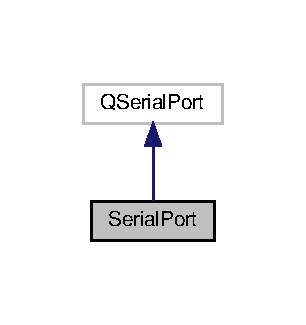
\includegraphics[width=147pt]{classSerialPort__inherit__graph}
\end{center}
\end{figure}


Collaboration diagram for Serial\+Port\+:\nopagebreak
\begin{figure}[H]
\begin{center}
\leavevmode
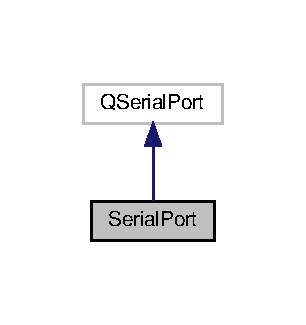
\includegraphics[width=147pt]{classSerialPort__coll__graph}
\end{center}
\end{figure}
\subsubsection*{Signals}
\begin{DoxyCompactItemize}
\item 
void \hyperlink{classSerialPort_a7313923f2de05683b56acce7c3bac7ff}{value\+Changed} (Q\+String str)
\end{DoxyCompactItemize}
\subsubsection*{Public Member Functions}
\begin{DoxyCompactItemize}
\item 
\hyperlink{classSerialPort_a193bce5b89cafd1e7ede389a0bf9295c}{Serial\+Port} (Q\+Object $\ast$parent=nullptr)
\begin{DoxyCompactList}\small\item\em Sets up basic stuff. \end{DoxyCompactList}\end{DoxyCompactItemize}
\subsubsection*{Private Slots}
\begin{DoxyCompactItemize}
\item 
void \hyperlink{classSerialPort_a0b8fe1371e829199856e8cae942de94e}{read\+Data} ()
\begin{DoxyCompactList}\small\item\em Gathers data bytes to commands. \end{DoxyCompactList}\end{DoxyCompactItemize}
\subsubsection*{Private Attributes}
\begin{DoxyCompactItemize}
\item 
Q\+String \hyperlink{classSerialPort_a2f94f65fcf6950d7e033d48077f0282d}{\+\_\+temp}
\item 
Q\+List$<$ Q\+String $>$ \hyperlink{classSerialPort_aa5417aaf7597e7b7349f9871a8dd5b2f}{\+\_\+list}
\end{DoxyCompactItemize}


\subsubsection{Constructor \& Destructor Documentation}
\mbox{\Hypertarget{classSerialPort_a193bce5b89cafd1e7ede389a0bf9295c}\label{classSerialPort_a193bce5b89cafd1e7ede389a0bf9295c}} 
\index{Serial\+Port@{Serial\+Port}!Serial\+Port@{Serial\+Port}}
\index{Serial\+Port@{Serial\+Port}!Serial\+Port@{Serial\+Port}}
\paragraph{\texorpdfstring{Serial\+Port()}{SerialPort()}}
{\footnotesize\ttfamily Serial\+Port\+::\+Serial\+Port (\begin{DoxyParamCaption}\item[{Q\+Object $\ast$}]{parent = {\ttfamily nullptr} }\end{DoxyParamCaption})}



Sets up basic stuff. 


\begin{DoxyParams}{Parameters}
{\em parent} & \\
\hline
\end{DoxyParams}


\subsubsection{Member Function Documentation}
\mbox{\Hypertarget{classSerialPort_a0b8fe1371e829199856e8cae942de94e}\label{classSerialPort_a0b8fe1371e829199856e8cae942de94e}} 
\index{Serial\+Port@{Serial\+Port}!read\+Data@{read\+Data}}
\index{read\+Data@{read\+Data}!Serial\+Port@{Serial\+Port}}
\paragraph{\texorpdfstring{read\+Data}{readData}}
{\footnotesize\ttfamily void Serial\+Port\+::read\+Data (\begin{DoxyParamCaption}{ }\end{DoxyParamCaption})\hspace{0.3cm}{\ttfamily [private]}, {\ttfamily [slot]}}



Gathers data bytes to commands. 

\mbox{\Hypertarget{classSerialPort_a7313923f2de05683b56acce7c3bac7ff}\label{classSerialPort_a7313923f2de05683b56acce7c3bac7ff}} 
\index{Serial\+Port@{Serial\+Port}!value\+Changed@{value\+Changed}}
\index{value\+Changed@{value\+Changed}!Serial\+Port@{Serial\+Port}}
\paragraph{\texorpdfstring{value\+Changed}{valueChanged}}
{\footnotesize\ttfamily void Serial\+Port\+::value\+Changed (\begin{DoxyParamCaption}\item[{Q\+String}]{str }\end{DoxyParamCaption})\hspace{0.3cm}{\ttfamily [signal]}}



\subsubsection{Member Data Documentation}
\mbox{\Hypertarget{classSerialPort_aa5417aaf7597e7b7349f9871a8dd5b2f}\label{classSerialPort_aa5417aaf7597e7b7349f9871a8dd5b2f}} 
\index{Serial\+Port@{Serial\+Port}!\+\_\+list@{\+\_\+list}}
\index{\+\_\+list@{\+\_\+list}!Serial\+Port@{Serial\+Port}}
\paragraph{\texorpdfstring{\+\_\+list}{\_list}}
{\footnotesize\ttfamily Q\+List$<$Q\+String$>$ Serial\+Port\+::\+\_\+list\hspace{0.3cm}{\ttfamily [private]}}

\mbox{\Hypertarget{classSerialPort_a2f94f65fcf6950d7e033d48077f0282d}\label{classSerialPort_a2f94f65fcf6950d7e033d48077f0282d}} 
\index{Serial\+Port@{Serial\+Port}!\+\_\+temp@{\+\_\+temp}}
\index{\+\_\+temp@{\+\_\+temp}!Serial\+Port@{Serial\+Port}}
\paragraph{\texorpdfstring{\+\_\+temp}{\_temp}}
{\footnotesize\ttfamily Q\+String Serial\+Port\+::\+\_\+temp\hspace{0.3cm}{\ttfamily [private]}}



The documentation for this class was generated from the following files\+:\begin{DoxyCompactItemize}
\item 
\hyperlink{SerialPort_8h}{Serial\+Port.\+h}\item 
\hyperlink{SerialPort_8cpp}{Serial\+Port.\+cpp}\end{DoxyCompactItemize}

\section{File Documentation}
\hypertarget{Chart_8cpp}{}\subsection{Chart.\+cpp File Reference}
\label{Chart_8cpp}\index{Chart.\+cpp@{Chart.\+cpp}}
{\ttfamily \#include \char`\"{}Chart.\+h\char`\"{}}\newline
Include dependency graph for Chart.\+cpp\+:
\nopagebreak
\begin{figure}[H]
\begin{center}
\leavevmode
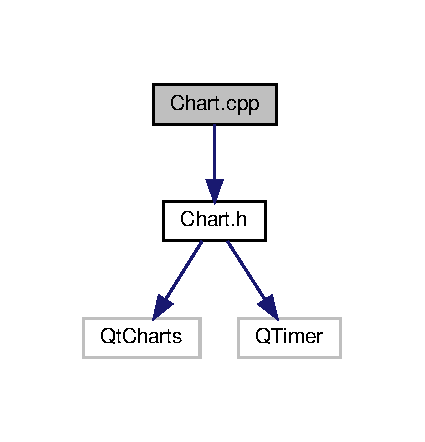
\includegraphics[width=204pt]{Chart_8cpp__incl}
\end{center}
\end{figure}

\hypertarget{Chart_8h}{}\subsection{Chart.\+h File Reference}
\label{Chart_8h}\index{Chart.\+h@{Chart.\+h}}
{\ttfamily \#include $<$Qt\+Charts$>$}\newline
{\ttfamily \#include $<$Q\+Timer$>$}\newline
Include dependency graph for Chart.\+h\+:
\nopagebreak
\begin{figure}[H]
\begin{center}
\leavevmode
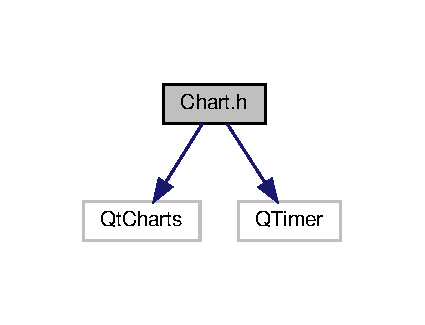
\includegraphics[width=204pt]{Chart_8h__incl}
\end{center}
\end{figure}
This graph shows which files directly or indirectly include this file\+:
\nopagebreak
\begin{figure}[H]
\begin{center}
\leavevmode
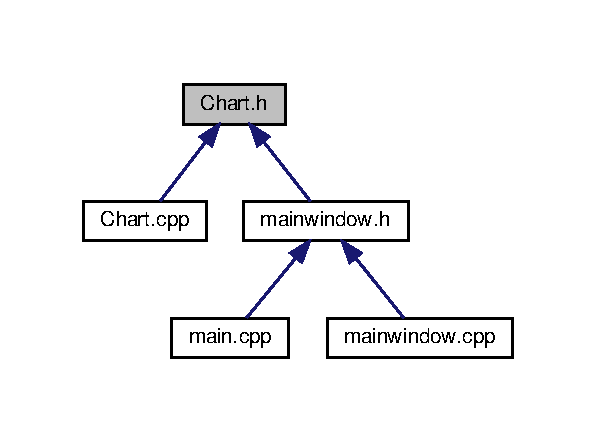
\includegraphics[width=286pt]{Chart_8h__dep__incl}
\end{center}
\end{figure}
\subsubsection*{Classes}
\begin{DoxyCompactItemize}
\item 
class \hyperlink{classChart}{Chart}
\end{DoxyCompactItemize}

\hypertarget{main_8cpp}{}\subsection{main.\+cpp File Reference}
\label{main_8cpp}\index{main.\+cpp@{main.\+cpp}}
{\ttfamily \#include \char`\"{}mainwindow.\+h\char`\"{}}\newline
{\ttfamily \#include $<$Qt\+Widgets$>$}\newline
{\ttfamily \#include $<$Q\+Application$>$}\newline
Include dependency graph for main.\+cpp\+:
\nopagebreak
\begin{figure}[H]
\begin{center}
\leavevmode
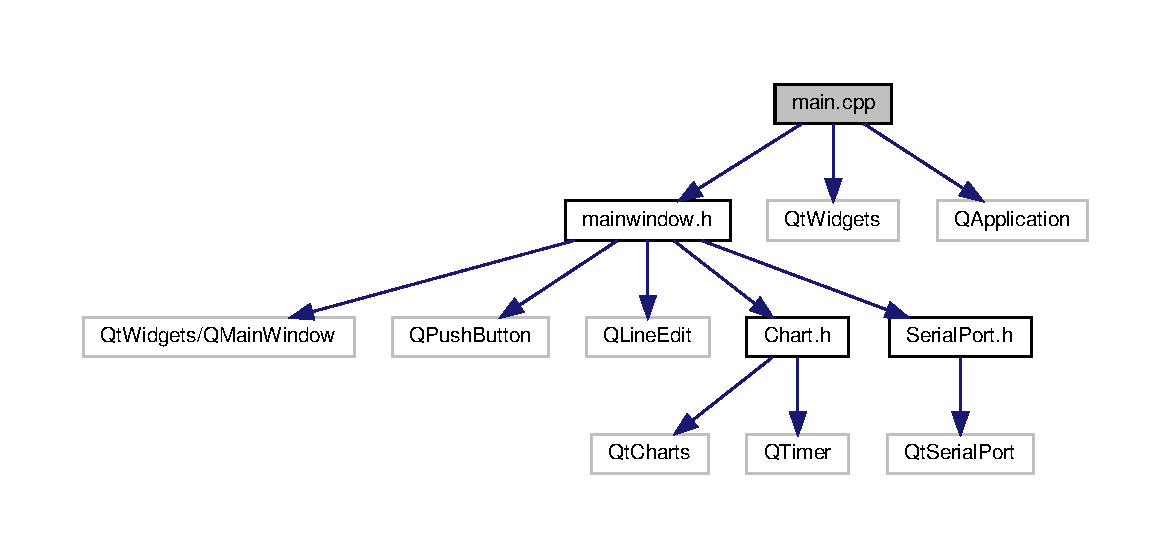
\includegraphics[width=350pt]{main_8cpp__incl}
\end{center}
\end{figure}
\subsubsection*{Functions}
\begin{DoxyCompactItemize}
\item 
int \hyperlink{main_8cpp_a0ddf1224851353fc92bfbff6f499fa97}{main} (int argc, char $\ast$argv\mbox{[}$\,$\mbox{]})
\end{DoxyCompactItemize}


\subsubsection{Function Documentation}
\mbox{\Hypertarget{main_8cpp_a0ddf1224851353fc92bfbff6f499fa97}\label{main_8cpp_a0ddf1224851353fc92bfbff6f499fa97}} 
\index{main.\+cpp@{main.\+cpp}!main@{main}}
\index{main@{main}!main.\+cpp@{main.\+cpp}}
\paragraph{\texorpdfstring{main()}{main()}}
{\footnotesize\ttfamily int main (\begin{DoxyParamCaption}\item[{int}]{argc,  }\item[{char $\ast$}]{argv\mbox{[}$\,$\mbox{]} }\end{DoxyParamCaption})}


\hypertarget{mainwindow_8cpp}{}\subsection{mainwindow.\+cpp File Reference}
\label{mainwindow_8cpp}\index{mainwindow.\+cpp@{mainwindow.\+cpp}}
{\ttfamily \#include \char`\"{}mainwindow.\+h\char`\"{}}\newline
{\ttfamily \#include $<$Q\+Grid\+Layout$>$}\newline
Include dependency graph for mainwindow.\+cpp\+:
\nopagebreak
\begin{figure}[H]
\begin{center}
\leavevmode
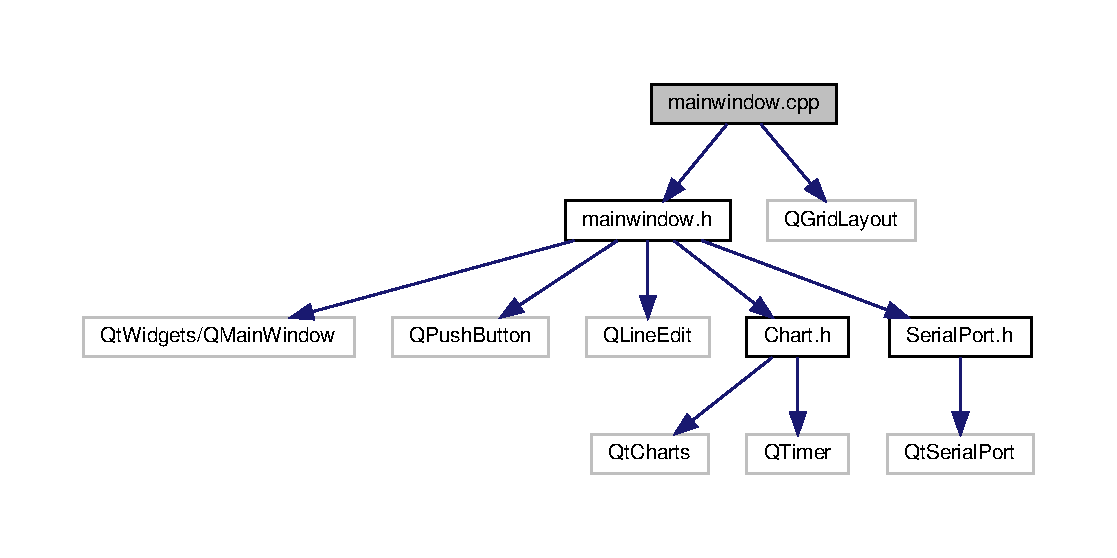
\includegraphics[width=350pt]{mainwindow_8cpp__incl}
\end{center}
\end{figure}

\hypertarget{mainwindow_8h}{}\subsection{mainwindow.\+h File Reference}
\label{mainwindow_8h}\index{mainwindow.\+h@{mainwindow.\+h}}
{\ttfamily \#include $<$Qt\+Widgets/\+Q\+Main\+Window$>$}\newline
{\ttfamily \#include $<$Q\+Push\+Button$>$}\newline
{\ttfamily \#include $<$Q\+Line\+Edit$>$}\newline
{\ttfamily \#include \char`\"{}Chart.\+h\char`\"{}}\newline
{\ttfamily \#include \char`\"{}Serial\+Port.\+h\char`\"{}}\newline
Include dependency graph for mainwindow.\+h\+:
\nopagebreak
\begin{figure}[H]
\begin{center}
\leavevmode
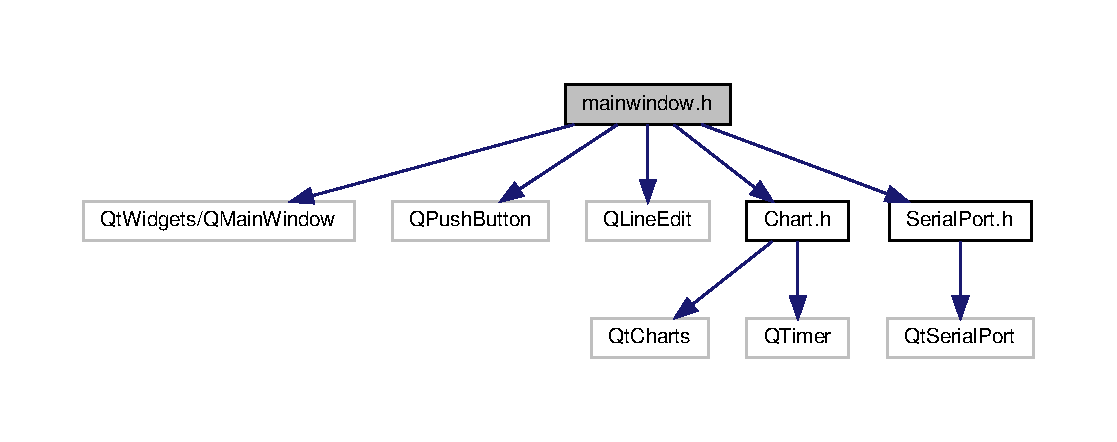
\includegraphics[width=350pt]{mainwindow_8h__incl}
\end{center}
\end{figure}
This graph shows which files directly or indirectly include this file\+:\nopagebreak
\begin{figure}[H]
\begin{center}
\leavevmode
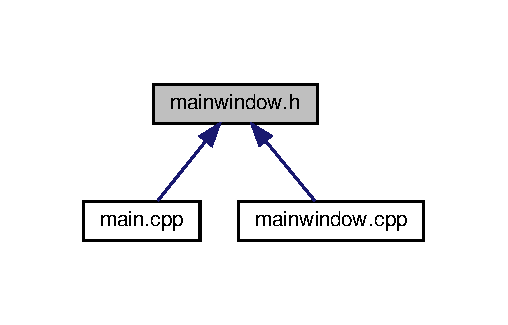
\includegraphics[width=244pt]{mainwindow_8h__dep__incl}
\end{center}
\end{figure}
\subsubsection*{Classes}
\begin{DoxyCompactItemize}
\item 
class \hyperlink{classMainWindow}{Main\+Window}
\end{DoxyCompactItemize}

\hypertarget{SerialPort_8cpp}{}\subsection{Serial\+Port.\+cpp File Reference}
\label{SerialPort_8cpp}\index{Serial\+Port.\+cpp@{Serial\+Port.\+cpp}}
{\ttfamily \#include \char`\"{}Serial\+Port.\+h\char`\"{}}\newline
Include dependency graph for Serial\+Port.\+cpp\+:\nopagebreak
\begin{figure}[H]
\begin{center}
\leavevmode
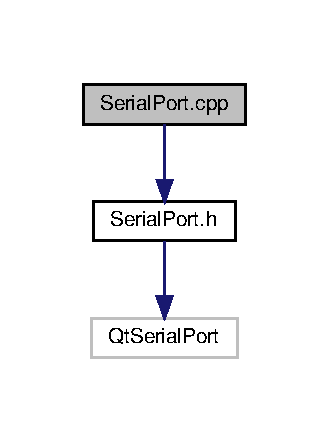
\includegraphics[width=158pt]{SerialPort_8cpp__incl}
\end{center}
\end{figure}

\hypertarget{SerialPort_8h}{}\subsection{Serial\+Port.\+h File Reference}
\label{SerialPort_8h}\index{Serial\+Port.\+h@{Serial\+Port.\+h}}
{\ttfamily \#include $<$Qt\+Serial\+Port$>$}\newline
Include dependency graph for Serial\+Port.\+h\+:\nopagebreak
\begin{figure}[H]
\begin{center}
\leavevmode
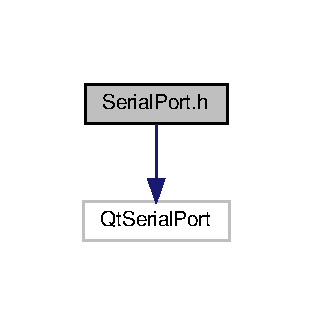
\includegraphics[width=150pt]{SerialPort_8h__incl}
\end{center}
\end{figure}
This graph shows which files directly or indirectly include this file\+:\nopagebreak
\begin{figure}[H]
\begin{center}
\leavevmode
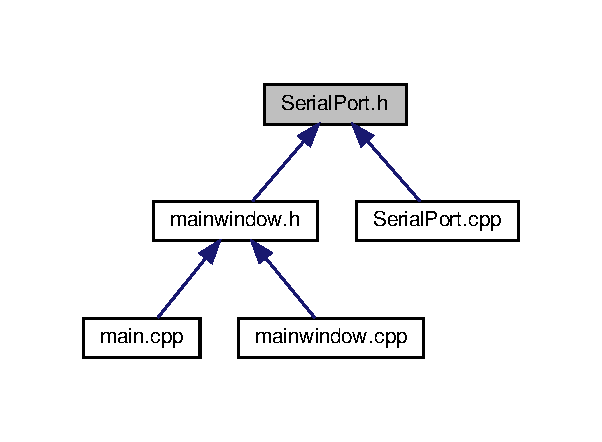
\includegraphics[width=289pt]{SerialPort_8h__dep__incl}
\end{center}
\end{figure}
\subsubsection*{Classes}
\begin{DoxyCompactItemize}
\item 
class \hyperlink{classSerialPort}{Serial\+Port}
\end{DoxyCompactItemize}

%--- End generated contents ---

% Index
\newpage
\phantomsection
\clearemptydoublepage
\addcontentsline{toc}{section}{Index}
\printindex

\end{document}
